\begin{center}
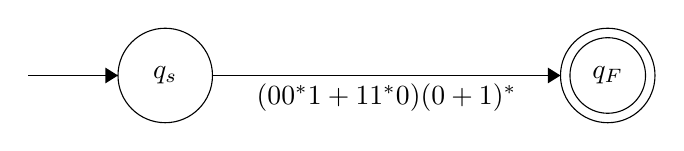
\begin{tikzpicture}[scale=0.2]
\tikzstyle{every node}+=[inner sep=0pt]
\draw [black] (54.2,-30.4) circle (3);
\draw (54.2,-30.4) node {$q_F$};
\draw [black] (54.2,-30.4) circle (2.4);
\draw [black] (26.1,-30.4) circle (3);
\draw (26.1,-30.4) node {$q_s$};
\draw [black] (17.4,-30.4) -- (23.1,-30.4);
\fill [black] (23.1,-30.4) -- (22.3,-29.9) -- (22.3,-30.9);
\draw [black] (29.1,-30.4) -- (51.2,-30.4);
\fill [black] (51.2,-30.4) -- (50.4,-29.9) -- (50.4,-30.9);
\draw (40.15,-30.9) node [below] {$(00^*1+11^*0)(0+1)^*$};
\end{tikzpicture}
\end{center}